 \documentclass[12pt,a4paper]{article}
\usepackage[utf8]{inputenc}
\usepackage[T1]{fontenc}
%\usepackage{gentium}
\usepackage{mathptmx} % Use Times Font

\usepackage{graphicx} % Required for including pictures
\usepackage{hyperref} % Format links for pdf
\usepackage{biblatex}
\addbibresource{references.bib}
\usepackage{booktabs} % Used so that tables generated by pandas
                      % to_latex() work correctly

\frenchspacing % No double spacing between sentences
\usepackage[margin=1in]{geometry}

\usepackage[all]{nowidow} % Tries to remove widows
\usepackage[protrusion=true,expansion=true]{microtype} % Improves typography, load after fontpackage is selected

\usepackage{lipsum} % Used for inserting dummy 'Lorem ipsum' text into the template
\usepackage{caption}
\usepackage{wrapfig}
\usepackage{float}
\usepackage{blindtext}


\title{Simple Heuristics for Path Integration in Ants}
\author{}

\begin{document}
\maketitle

\section*{Abstract}

Ants exhibit remarkable navigational abilities, often returning to their nests after foraging using a combination of path integration and visual cues. This report presents a computationally plausible model that combines a simulated solar compass with visual landmark recognition, inspired by the ant's mushroom body (MB) neural architecture. We developed and tested three navigation strategies: using only a solar compass, using only visual cues processed through the MB network, and a combined approach utilising both methods. Our experiments measured the computational efficiency of each strategy. The results demonstrate that the combined navigation strategy significantly improves efficiency, achieving faster training and testing times compared to using visual cues alone, while also providing more reliable homing behaviour than relying solely on the solar compass. These findings suggest that ants likely employ a combined navigational strategy.

\\~\\
\section{Introduction}
% Suggested 400 words

Animals employ various methods to navigate back to their homes after foraging. One of the most widespread strategies is path integration. Path integration allows animals to maintain an estimate of their location relative to a frame of reference, such as a fixed nest position. This navigation system enables creatures to generate a homeward-pointing vector, facilitating a direct return to their nest or hive \cite{wehner_2008}.

The process of path integration in insects involves continuously tracking the distance covered and the direction of travel during their outbound journey. This information is integrated over time, creating a return vector. The resulting vector provides both the straight-line distance to the starting point and the direction for a direct return. Insects rely on a solar compass for this path integration process, allowing them to maintain directional consistency even over long distances \cite{wehner_2008}.

The solar compass enables insects to determine direction based on celestial cues such as the position of the sun or patterns of polarised light in the sky. This system works in conjunction with an internal odometer that helps them measure the distance travelled \cite{wehner_2008} . By combining these two mechanisms, insects can accurately track their movements and calculate an efficient route back to their home base. A celestial compass uses the properties of light coming from the sky to estimate the position of the primary celestial body or with appropriate time compensation, the North \cite{gkanias_mitchell_stankiewicz_khan_mitra_webb_2023}. 

Ants don't rely solely on path integration for navigation. They have also been observed using visual cues and landmarks to guide their movements \cite{collett_graham_harris_2007, zeil_2012}. This visual-based navigation system operates independently of path integration.

The neural mechanisms underlying path integration in insects, particularly ants, have been a subject of considerable debate. Despite extensive research, the precise neural pathways responsible for this navigational ability remain unknown. 

In light of these various navigational methods, we hypothesise that ants employ a combined strategy, integrating both a solar compass and visual cues to navigate back to their nest after foraging. This approach allows insects to navigate effectively under various conditions, whether in open terrain where celestial cues are readily available or in more cluttered environments where visual landmarks become crucial.

\\~\\
\section{Architecture of the Navigational Model}

\paragraph{Mushroom Body}\\~\\
The visual processing in ant brains shares similarities with other insects in its initial sensory layers \cite{ardin_peng_mangan_lagogiannis_webb_2016}. Ants have compound eyes with varying resolution across species. For desert ants like \textit{Cataglyphis} \cite{zollikofer_wehner_fukushi_1995} and \textit{Melaphorus bagoti} \cite{schwarz_narendra_zeil_2011}, the eyes cover a wide field of vision but with low resolution. Visual signals pass through the optic lobe while maintaining a retinotopic projection, then go to the protocerebrum, central complex, and mushroom bodies (MB) \cite{ehmer_gronenberg_2003}. The MB is notably involved in visual learning and navigation in ants, unlike in other insects where it primarily processes olfactory inputs \cite{schürmannfw_1970}.

While the MB is usually studied for its role in olfactory learning, evidence suggests it also plays a part in visual learning \cite{heisenberg_2003}. Previous models of olfactory learning in \textit{Drosophila} show how sensory input is sparsely encoded in the MB, allowing for reward-based learning \cite{cassenaer_laurent_2012}. This same circuit model can be applied to visual learning in ants, enabling them to associate visual patterns seen during navigation with reaching a goal, like returning home.

The mushroom body used for the visual cue mechanism is similar to \cite{wessnitzer_young_armstrong_webb_2011}. The only difference was the increase of the number of neurons, but still under the estimates for the number of neurons in ants \cite{ehmer_gronenberg_2003}, and also using anti-Hebbian learning, similar to the one used by \cite{ardin_peng_mangan_lagogiannis_webb_2016}. 

The mushroom body model consists of three layers. The input layer comprises of 360 visual projection neurons (vPNs), whose signals are scaled and normalized. The second layer contains 20,000 Kenyon cells (KCs), each receiving input from 10 randomly selected vPNs. This sparse, random connectivity helps in the decorrelation of visual information, allowing for more efficient encoding of images using sparse representations \cite{laurent_2002}. The output of all KCs converges onto a single extrinsic neuron (EN). Over time, repeated learning to similar images weakens the connections between the corresponding vPNs and KCs, reducing the activation of KCs for learned images.

\begin{figure}[H]
    \centering
    \captionsetup{justification=centering, margin=2cm}
    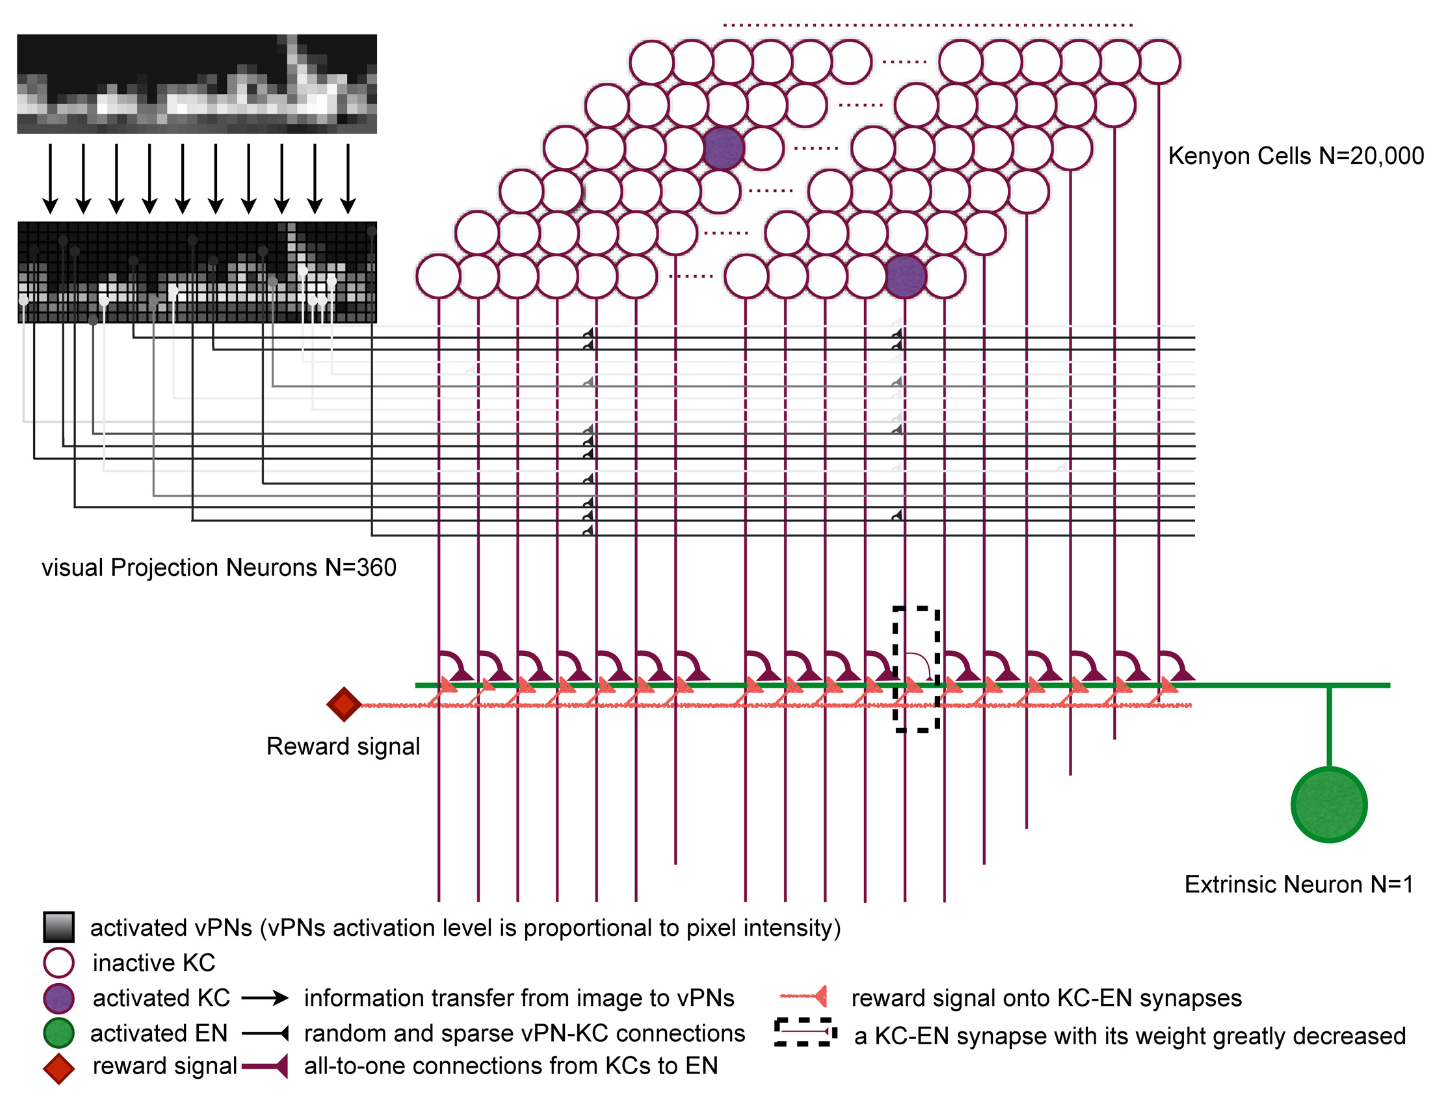
\includegraphics[width=.8\linewidth]{mb_model.png}
    \caption{\textbf{Architecture of the Mushroom Body (MB) model} \cite{ardin_peng_mangan_lagogiannis_webb_2016}}
    \label{mb_model}
\end{figure}
\\~\\

\paragraph{Solar Compass}\\~\\
\begin{wrapfigure}{i}{.5\textwidth}
    \begin{center}
    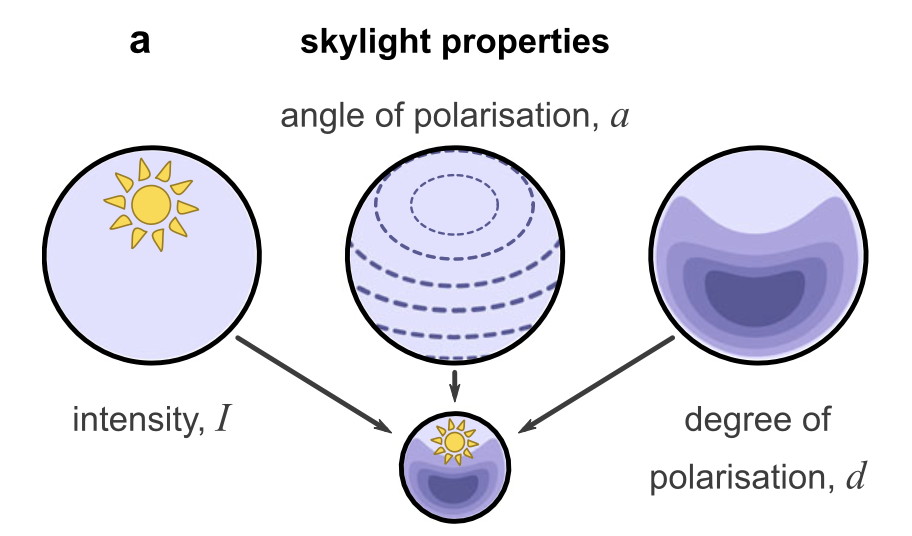
\includegraphics[width=.8\linewidth]{skylight_prop.png}
    \end{center}
    \captionsetup{justification=centering,margin=0cm}
    \caption{\textbf{Skylight properties used for insect navigation} \cite{gkanias_mitchell_stankiewicz_khan_mitra_webb_2023}}
    \label{mb_model}
\end{wrapfigure}
Insects use the position of the sun as a navigational compass, filtering celestial light intensity and polarisation through their compound eyes. Light from large celestial objects, such as the sun, creates a predictable pattern of intensity and polarisation across the sky. Under clear conditions, the intensity of skylight peaks at the visual location of the sun \cite{wehner_2008}. The degree of polarisation is strongest in the opposite direction, at 90 degrees from the sun across the zenith. At any given point, the angle of polarisation is always perpendicular to the arc between the sun and that point, forming concentric rings of polarisation centered around the sun's position \cite{gkanias_mitchell_stankiewicz_khan_mitra_webb_2023}.

In our simulation, instead of modeling sunlight directly, we approximate this by summing the distance travelled and calculate both the distance and angle for returning to the nest. We introduced a Gaussian error of 2 degrees to the return angle to simulate error.


\section{Experiment Setup and Results}

\paragraph{Experiment Setup}\\~\\
In our experiment, we aimed to simulate an environment that closely mimics the foraging behaviour of ants. We based our simulation on the work and datasets of \cite{ardin_peng_mangan_lagogiannis_webb_2016}, which provided a comprehensive simulated environment.

The ground in our simulation is flat and featureless, and the sky is uniform without intensity or polarised light gradients. The ants’ visual input is reconstructed from a height of 1 cm above the ground, with a field of view that extends horizontally for 296 degrees and vertically for 76 degrees. With a resolution of 4 degrees per pixel, this setup produces a 19×74 pixel image. The image is then inverted in intensity, histogram equalised, and further down sampled to 10×36 pixels for input to the mushroom body (MB) network.

\begin{figure}[htbp]
    \centering
    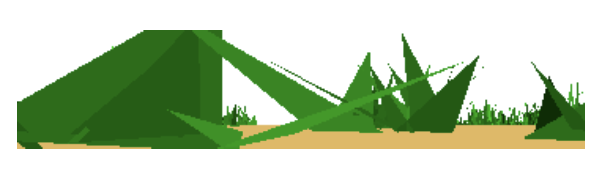
\includegraphics[width=0.5\linewidth]{a.png}
    \caption{Ant’s view of the environment.}
    \label{fig:ant_view}
\end{figure}

Using this data, we observed that ants typically follow a back-and-forth pattern between their nest and a specific foraging point \ref{ant_route}. To accurately represent the visual information available to ants, we captured a series of images around the nest, all facing towards the nest itself. These images were taken at multiple radii from the nest: 0.5, 0.3, and 0.2 metres. In total, we collected 170 images to train our neural network, providing a dataset of visual cues for the mushroom body model to learn from.

\begin{figure}[htbp]
    \centering
    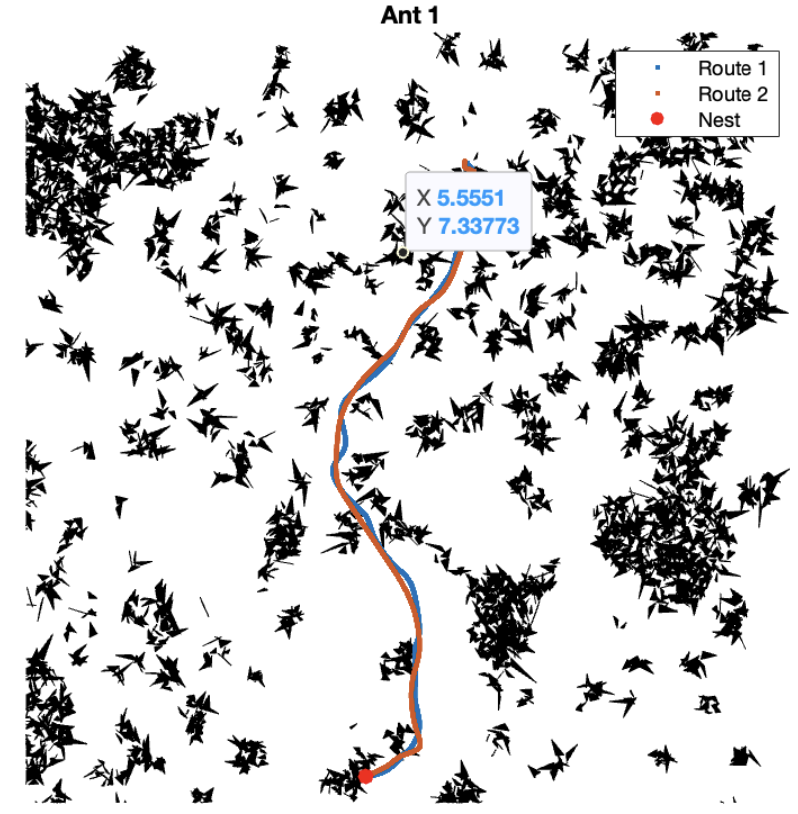
\includegraphics[width=0.4\linewidth]{ant_route.png}
    \caption{Example of an ant's route}
    \label{ant_route}
\end{figure}

Our experimental design incorporates both a solar compass and visual cues, reflecting our hypothesis that ants utilise a combination of these navigation methods. The solar compass was simulated by providing each virtual ant with a vector pointing back to the nest, guiding the ant’s initial direction of travel. To account for real-world variability and uncertainty in solar compass accuracy, we introduced a simulated error to the homing angle.

As the ants approach the vicinity of their nest, the navigation system in our simulation switches from primarily relying on the solar compass to utilising visual cues. This transition mimics the behaviour we hypothesise occurs in real ants when they are near familiar territory.

From extensive testing, we determined that when using visual cues, the ant should move towards a certain direction when the output neuron value is below 8. This threshold was established based on the neural network’s responses to images similar to those it was trained on versus unrelated images. If no image produces an output neuron value below 8, the ant continues in its previous direction \ref{en_output}.

\begin{figure}[H]
    \centering
    \captionsetup{justification=centering, margin=2cm}
    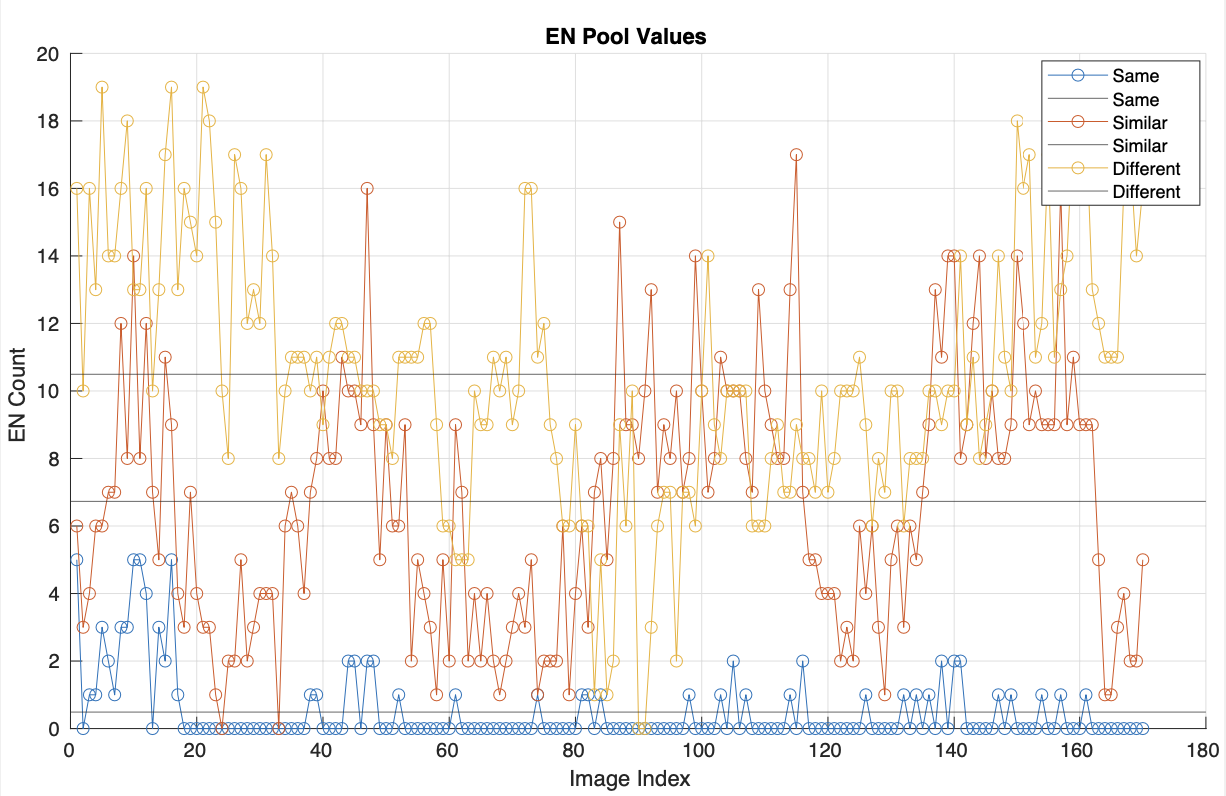
\includegraphics[width=1\linewidth]{enoutput.png}
    \caption{\textbf{Output neuron values for various images}}
    \label{en_output}
\end{figure}

\\~\\
\paragraph{Experiment Result}\\~\\
To evaluate the effectiveness of our navigation model, we conducted simulations under three different navigation strategies:

\begin{enumerate}
    \item Solar Compass Only: The ant relies solely on the solar compass for navigation.
    \item Visual Cues Only: The ant uses only visual cues processed through the mushroom body network.
    \item Combined Navigation: The ant uses both the solar compass and visual cues for navigation.
\end{enumerate}

For each strategy, we measured:

\begin{itemize}
    \item \textbf{Average Training Time}: The time required to train the model for the given navigation strategy.
    \item \textbf{Average Testing Time}: The time taken to run the simulation for each strategy.
\end{itemize}

The results are as follows:

\begin{table}[H]
    \centering
    \caption{Training and Testing Times for Different Navigation Strategies}
    \label{tab:times}
    \begin{tabular}{lcc}
        \toprule
        \textbf{Navigation Strategy} & \textbf{Training Time} & \textbf{Testing Time} \\
        \midrule
        Solar Compass Only & $<$1 second & $<$1 second \\
        Visual Cues Only & 1 minute 4 seconds & 10 minutes \\
        Combined Navigation & 1 minute 2 seconds & 1 minute 15 seconds \\
        \bottomrule
    \end{tabular}
\end{table}

\begin{figure}[H]
    \centering
    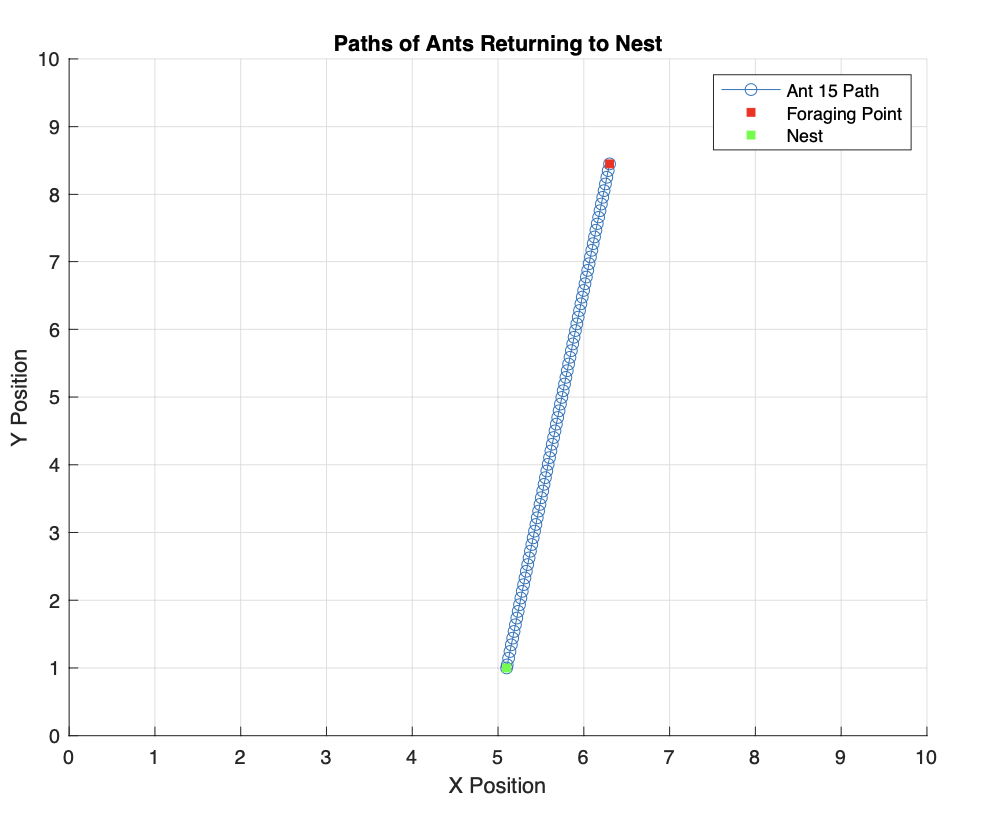
\includegraphics[width=0.5\linewidth]{pure_vector.png}
    \caption{\textbf{Navigation path using only the Solar Compass}. The ant follows a relatively straight path but may miss the nest due to accumulated errors.}
    \label{fig:solar_compass_only}
\end{figure}

\begin{figure}[H]
    \centering
    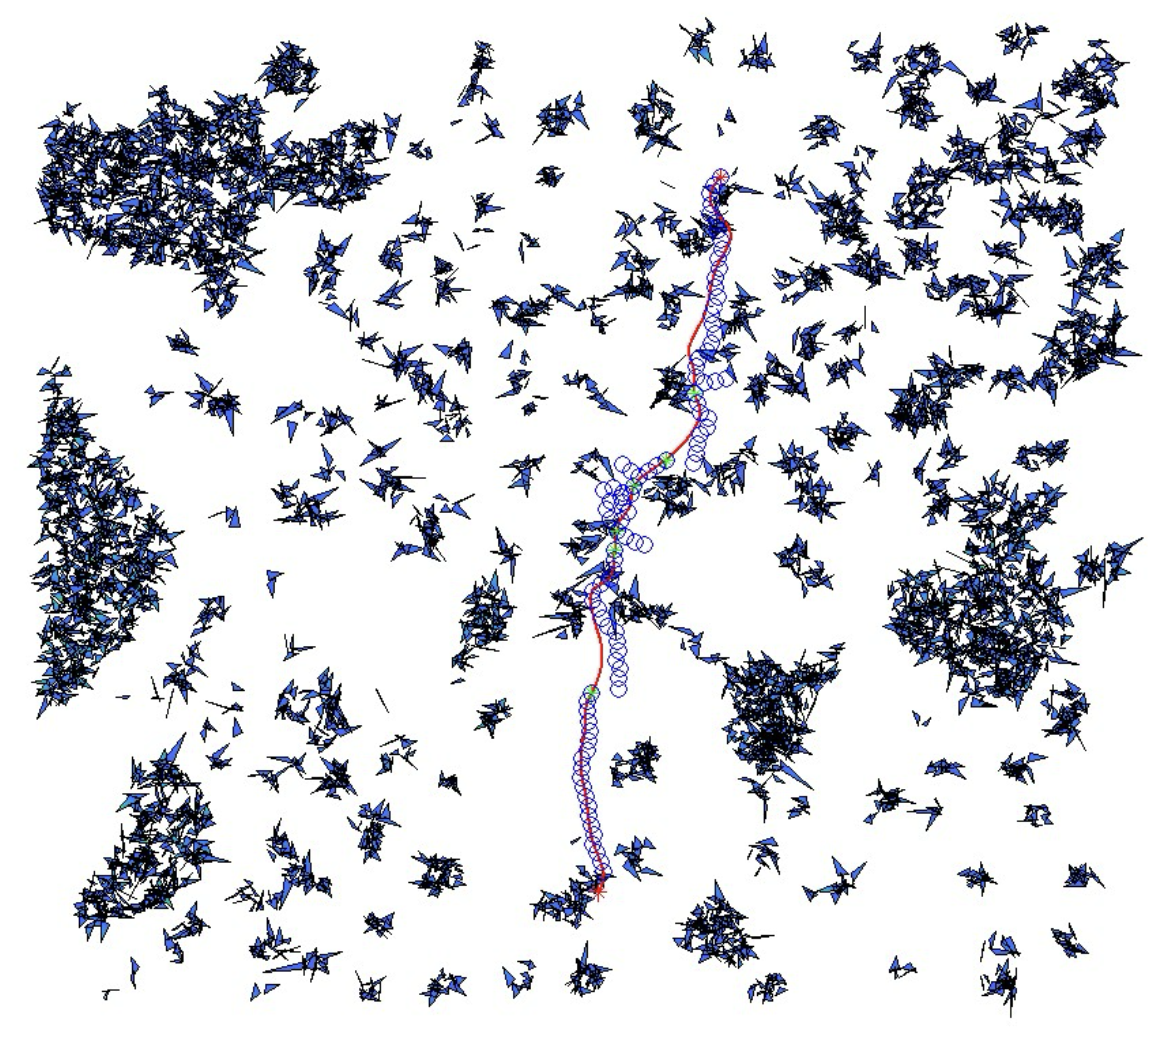
\includegraphics[width=0.5\linewidth]{pure_visual.png}
    \caption{\textbf{Navigation path using only visual cues}. The ant frequently snaps back to the route when it deviates off route, as indicated by the green circles. This indicates a significant amount of snapping back due to reliance on visual cues.}
    \label{fig:visual_cues_only}
\end{figure}

\begin{figure}[H]
    \centering
    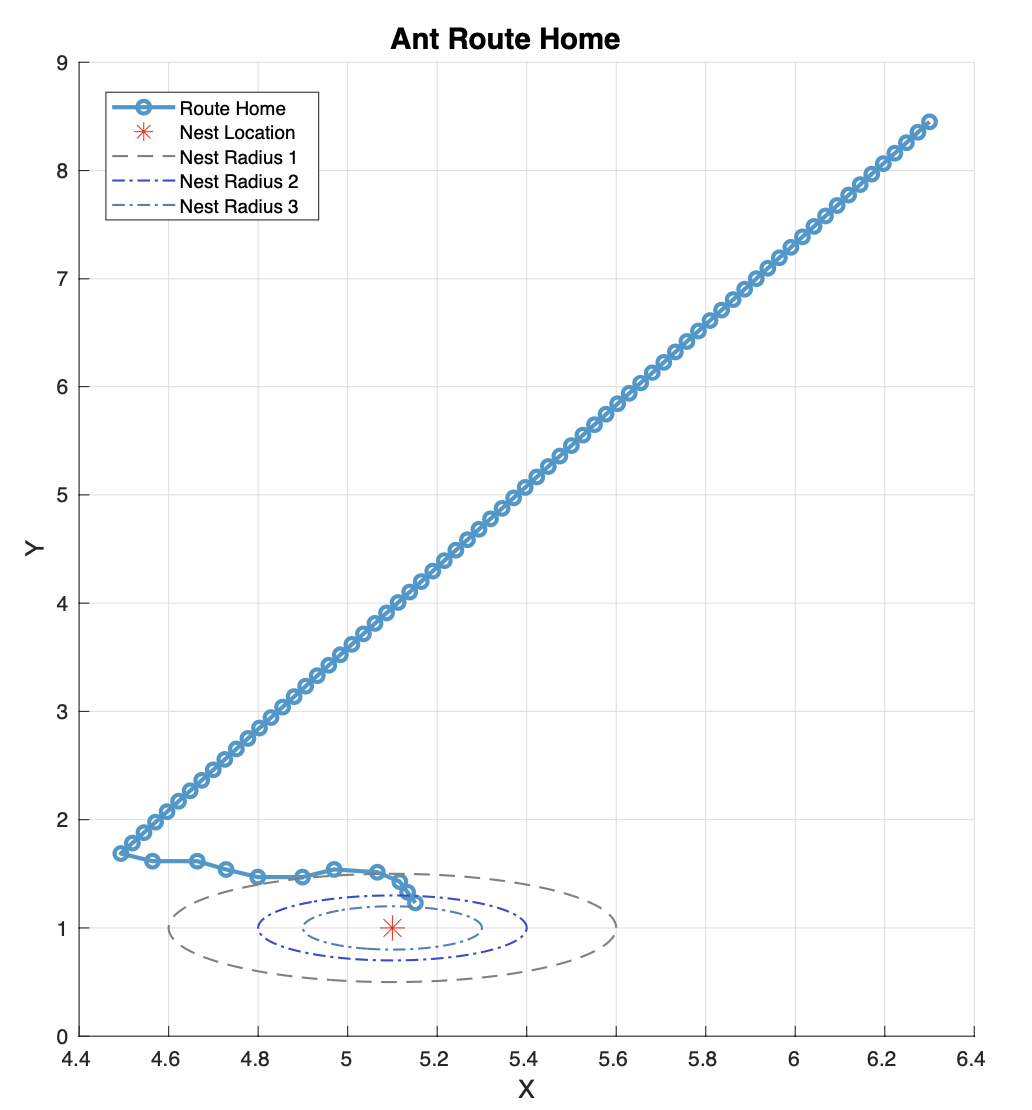
\includegraphics[width=0.5\linewidth]{both.png}
    \caption{\textbf{Navigation path using the combined navigation strategy}. The ant efficiently returns to the nest by combining solar compass guidance with visual cue recognition.}
    \label{fig:combined_navigation}
\end{figure}

\\~\\
\section{Discussion and conclusions}

Our experiments focused on evaluating the computational efficiency of different navigation strategies in ants, specifically analysing the training and testing times required for each method. The results presented in Table~\ref{tab:times} reveal significant differences in computational demands among the strategies.

The Solar Compass Only strategy is the most computationally efficient, with both training and testing times being less than one second. This is expected since the solar compass model involves simple vector calculations without the need for complex neural network processing. However, this strategy lacks robustness in environments with errors.

The visual cues only strategy requires considerably more computational resources, with a training time of 1 minute and 6 seconds and a testing time of 10 minutes. The increased testing time is attributed to the complexity of processing visual information through the mushroom body network.

The combined navigation strategy strikes a balance between computational efficiency and navigational robustness. It has a training time of 1 minute and 2 seconds and a testing time of 1 minute and 15 seconds. By integrating both the solar compass and visual cues, the model benefits from the quick directional guidance of the solar compass and the precise landmark recognition of the visual system, without the high computational cost seen in the visual cues only strategy.

These findings suggest that ants may utilise a combined navigation approach not only for effectiveness but also for computational efficiency. The use of multiple navigational strategies allows for a more reliable homing behaviour with low energy and time costs.

\printbibliography
\end{document}